\section{Test af hardware}
\subsection{Modultest}

\subsection{Integrationstest}
Formålet med at lave en integrationstest er at teste at de forskellige moduler virker, når de integreres. Vi ønsker at undersøge hvilke outputs de forskellige tryk på vandsøjlen giver, og derved se om der er en sammenhæng mellem tryk og spænding.

Der blev udført en række tests, hvor hele systemet var koblet sammen. Vi undersøgte hvilke spændinger vores system ville give ved et tryk på henholdsvis 100 mmHg, 50 mmHg og 10 mmHg.  Fra WaveForms gav vi subtraktoren 2 V, og resten af systemet fik +5 og -5 V. I intergretionstesten ville vi forvente at vores spændinger ville ligger inden for et interval der hedder + 2 og - 2 V, da subtraktoren nedsænker signalet med 2V.

\vspace{0.5 cm}

\begin{figure}[h!]
	\centering
	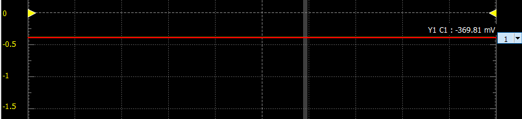
\includegraphics[width=0.75\linewidth]{../Rapport/Implementering_og_test/Hardware/integration100mmhg}
	\caption{Integrationstest med vandsøjle - 100 mmHg}
	\label{fig:i100mmhg}
\end{figure}

\begin{figure}[h!]
	\centering
	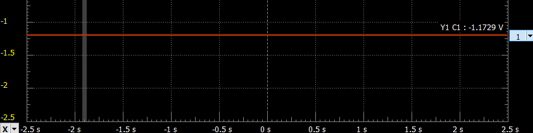
\includegraphics[width=0.75\linewidth]{../Rapport/Implementering_og_test/Hardware/integration50mmhg}
	\caption{Integrationstest med vandsøjle - 50 mmHg}
	\label{fig:i50mmhg}
\end{figure}

\begin{figure}[h!]
	\centering
	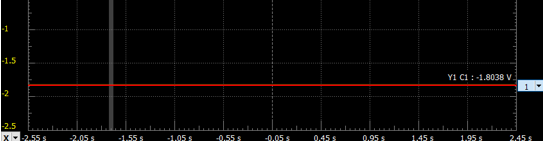
\includegraphics[width=0.75\linewidth]{../Rapport/Implementering_og_test/Hardware/integration10mmhg}
	\caption{Integrationstest med vandsøjle - 10 mmHg}
	\label{fig:i10mmgh}
\end{figure}

\begin{figure}[h!]
	\centering
	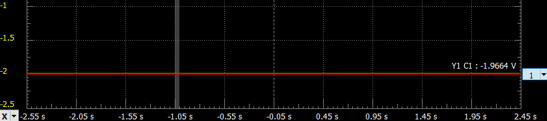
\includegraphics[width=0.75\linewidth]{../Rapport/Implementering_og_test/Hardware/integration0mmhg}
	\caption{Integrationstest med vandsøjle - 0 mmHg}
	\label{fig:i0mmhg}
\end{figure}

\clearpage

Vi ved at vandsøjlen er 1360 mm høj ved et tryk på 100 mmHg. Denne information kunne vi benytte til at udregne nogle andre tryk ved at ændre på vandhøjden i søjlen.
Der ønskes at undersøge trykket for 25 mmHg og 75 mmHg, hvilket er beregnet på følgende måde:

1360 * 0,25 = 340 mm
1360 * 0,75 = 1020,0 mm

Vi tilsluttede transduceren til vandsøjlen, og påfyldte vand i søjlen til de beregnede højder.

\begin{figure}[h!]
	\centering
	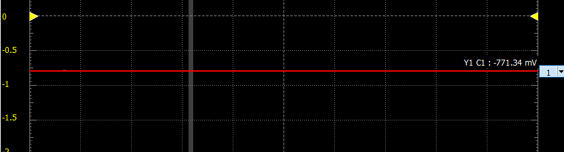
\includegraphics[width=0.75\linewidth]{../Rapport/Implementering_og_test/Hardware/integration75mmhg}
	\caption{Integrationstest med vandsøjle - 75 mmHg}
	\label{fig:i75mmgh}
\end{figure}

\begin{figure}[h!]
	\centering
	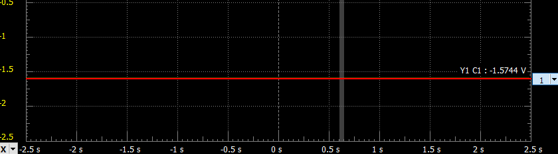
\includegraphics[width=0.75\linewidth]{../Rapport/Implementering_og_test/Hardware/integration25mmhg}
	\caption{Integrationstest med vandsøjle - 25 mmHg}
	\label{fig:i25mmhg}
\end{figure}

Tager vi alle vores målinger og plotter dem, ses der en tydelig sammenhæng mellem tryk og spænding.

\vspace{0.5 cm}

\begin{figure}[h!]
	\centering
	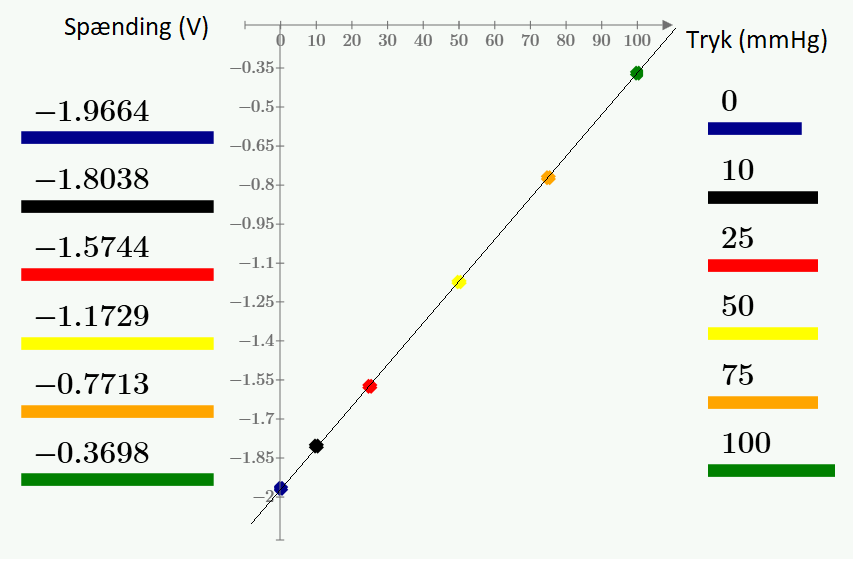
\includegraphics[width=0.75\linewidth]{../Rapport/Implementering_og_test/Hardware/integrationsplothw}
	\caption{Sammenhæng mellem tryk og spænding}
	\label{fig:iplot}
\end{figure}

\clearpage